\documentclass[10pt]{article}
\usepackage[letterpaper,margin=.8in]{geometry}
\usepackage[T1]{fontenc}
\usepackage{lmodern}
\usepackage{amsmath,amssymb,booktabs,tabularx,array,microtype}
\usepackage{tikz}
\usetikzlibrary{arrows.meta,positioning,fit,backgrounds,calc,shapes.geometric}
\usepackage[hidelinks]{hyperref}
\usepackage{caption}
\captionsetup{font=small,labelfont=bf,hypcap=false}
\setlength{\parindent}{0pt}
\setlength{\parskip}{4pt}
\newcolumntype{Y}{>{\raggedright\arraybackslash}X}
\newcommand{\code}[1]{\texttt{\small\detokenize{#1}}}
\newcommand{\Normal}{\mathcal N}
\newcommand{\logit}{\operatorname{logit}}
\newcommand{\repo}[2]{\href{../../../#1}{#2}}
\tikzset{
  latent/.style={circle,draw=black,line width=.5pt,fill=white,
    minimum size=10mm,inner sep=1pt,font=\small},
  observed/.style={latent,fill=black!15},
  shared/.style={latent,dashed,fill=black!3},
  bundle/.style={latent,ellipse,minimum width=19mm},
  derived/.style={latent,double,double distance=1pt},
  plate/.style={draw=black!45,rounded corners=2pt,inner sep=3mm,line width=.4pt},
  ptag/.style={font=\scriptsize\itshape,text=black!65,fill=white,inner sep=1pt},
  ed/.style={-{Stealth[length=1.8mm,width=1.4mm]},draw=black!65,line width=.5pt},
  box/.style={draw=black!65,rounded corners=2pt,align=center,inner sep=6pt,
    font=\small,text width=45mm},
  note/.style={font=\scriptsize,align=center,text=black!65}
}
\title{Implemented Bayesian architectures: v4 and v5}
\author{Companion to the simplified process--evidence model}
\date{Implementation snapshot: September 16, 2026}

\begin{document}
\maketitle
\vspace{-1em}

\section{One intended system; two research implementations}
The intended system infers a process and its burden from heterogeneous, imperfect
evidence, retaining posterior uncertainty. The existing
\href{generative_model.pdf}{simplified graphical model} is that broader target.
It is \emph{not} a statement that every node is implemented or identified.

\textbf{V4} is the agency/task/process hierarchy prototype. \textbf{V5} is a
smaller, process-level timing measurement prototype built to diagnose clock,
selection, outcome and partial-span errors. They share an evidence contract and
inference utilities, but are \emph{separate fitted models}. V5 is not a posterior
layer on top of v4, and it does not currently update v4's agency parameters.

\begin{center}
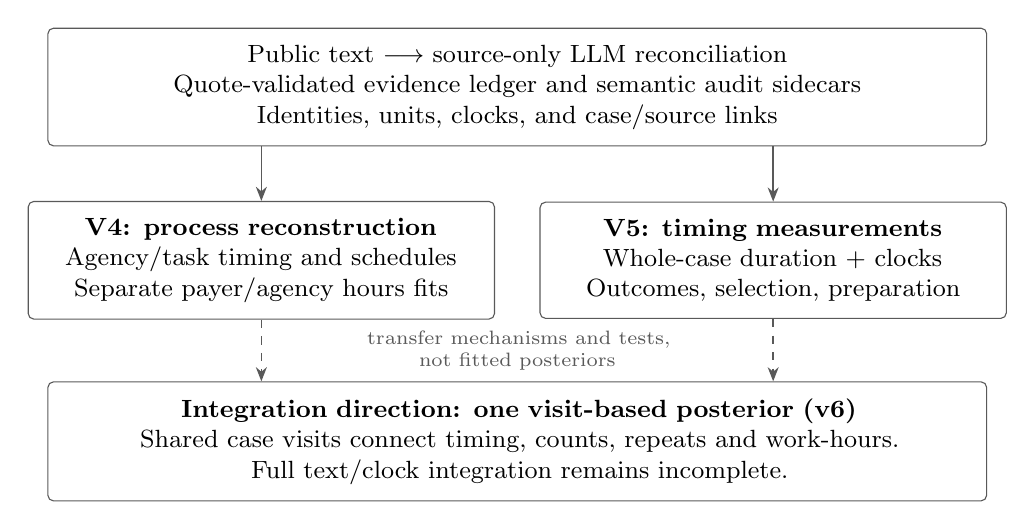
\begin{tikzpicture}[x=1cm,y=1cm]
  \node[box,text width=115mm] (ledger) at (0,0)
    {Public text $\longrightarrow$ source-only LLM reconciliation\\
     Quote-validated evidence ledger and semantic audit sidecars\\
     Identities, units, clocks, and case/source links};
  \node[box,text width=55mm] (v4) at (-3.25,-2.2)
    {\textbf{V4: process reconstruction}\\
     Agency/task timing and schedules\\
     Separate payer/agency hours fits};
  \node[box,text width=55mm] (v5) at (3.25,-2.2)
    {\textbf{V5: timing measurements}\\
     Whole-case duration $+$ clocks\\
     Outcomes, selection, preparation};
  \draw[ed] (ledger.south -| v4.north) -- (v4.north);
  \draw[ed] (ledger.south -| v5.north) -- (v5.north);
  \node[box,text width=115mm] (v6) at (0,-4.5)
    {\textbf{Integration direction: one visit-based posterior (v6)}\\
     Shared case visits connect timing, counts, repeats and work-hours.\\
     Full text/clock integration remains incomplete.};
  \draw[ed,dashed] (v4.south) -- (v6.north -| v4.south);
  \draw[ed,dashed] (v5.south) -- (v6.north -| v5.south);
  \node[note,fill=white,text width=50mm] at (0,-3.35)
    {transfer mechanisms and tests,\\not fitted posteriors};
\end{tikzpicture}
\end{center}

\begin{tabularx}{\linewidth}{@{}p{.28\linewidth}YY@{}}
\toprule Question & V4 & V5 \\
\midrule
How long does the process take? & Schedule of uncertain operations & Direct distribution of whole-case time \\
Can evidence inform an agency? & Yes, through shared agency/task effects & No agency/task parameters \\
How many steps or agencies? & Finite schedules and unseen-stage sensitivity; actor identities conditioned on reconciliation & Not estimated \\
What is the work burden? & Separate payer-hours and agency-hours fits & Not estimated \\
\bottomrule
\end{tabularx}

The LLM is an interpretation instrument here, not the numeric estimator. A direct
LLM baseline receives matched evidence in separate evaluations. Neither a passing
sampler diagnostic nor a favorable development score establishes superiority.

\clearpage
\section{V4: jointly learn timing and its hierarchical attribution}
\label{sec:v4}
The elapsed-time fit connects a step report and its case's process total to the
\emph{same} latent durations. Shared agency and task effects allow information to
move between operations and programs. The schematic below conditions on resolved
identities and source-supported metadata; it is not a model of raw text generation.

\begin{center}
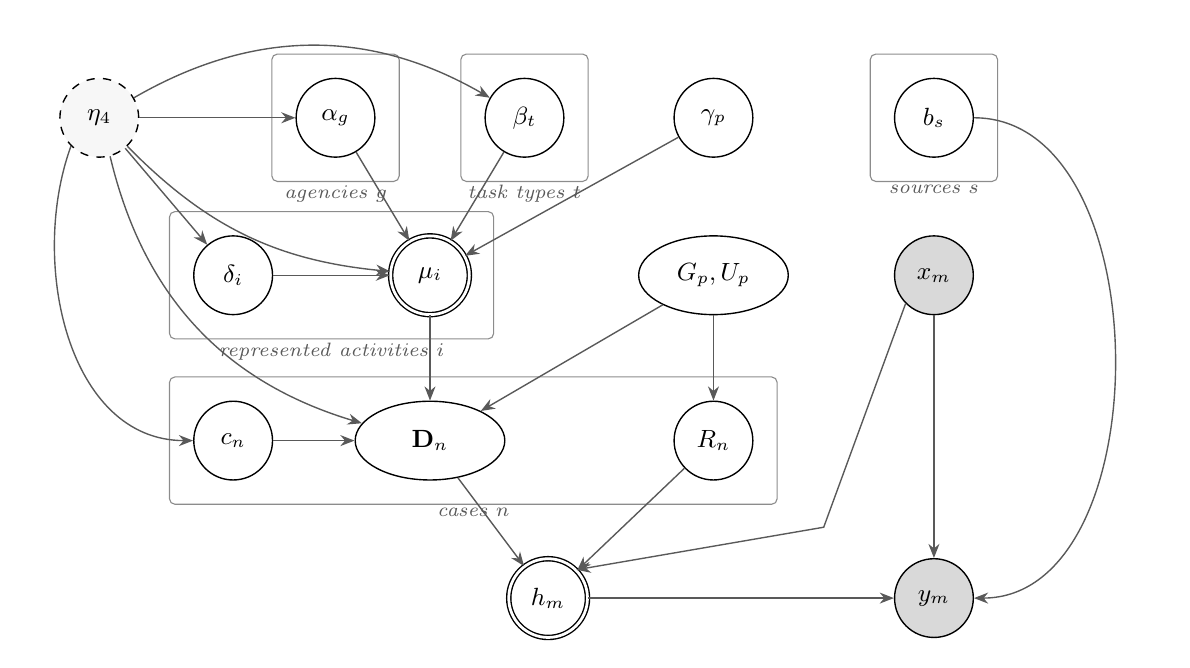
\begin{tikzpicture}[x=1cm,y=1cm]
  \node[shared] (eta) at (0,2.7) {$\eta_4$};
  \node[latent] (alpha) at (3.0,2.7) {$\alpha_g$};
  \node[latent] (beta) at (5.4,2.7) {$\beta_t$};
  \node[latent] (gamma) at (7.8,2.7) {$\gamma_p$};
  \node[latent] (source) at (10.6,2.7) {$b_s$};
  \node[latent] (delta) at (1.7,.7) {$\delta_i$};
  \node[derived] (mu) at (4.2,.7) {$\mu_i$};
  \node[bundle] (graph) at (7.8,.7) {$G_p,U_p$};
  \node[observed] (meta) at (10.6,.7) {$x_m$};
  \node[latent] (case) at (1.7,-1.4) {$c_n$};
  \node[bundle] (duration) at (4.2,-1.4) {$\mathbf D_n$};
  \node[latent] (route) at (7.8,-1.4) {$R_n$};
  \node[derived] (operator) at (5.7,-3.4) {$h_m$};
  \node[observed] (report) at (10.6,-3.4) {$y_m$};
  \begin{scope}[on background layer]
    \node[plate,fit=(alpha)] (ap) {};
    \node[plate,fit=(beta)] (tp) {};
    \node[plate,fit=(source)] (sp) {};
    \node[plate,fit=(delta)(mu)] (ip) {};
    \node[plate,fit=(case)(duration)(route)] (np) {};
  \end{scope}
  \node[ptag,anchor=north] at (ap.south) {agencies $g$};
  \node[ptag,anchor=north] at (tp.south) {task types $t$};
  \node[ptag,anchor=north] at (sp.south) {sources $s$};
  \node[ptag,anchor=north] at (ip.south) {represented activities $i$};
  \node[ptag,anchor=north] at (np.south) {cases $n$};
  \draw[ed] (eta) -- (alpha);
  \draw[ed] (eta) to[bend left=30] (beta);
  \draw[ed] (eta) -- (delta);
  \draw[ed] (eta) to[bend right=20] (mu);
  \draw[ed] (eta) to[bend right=30] (duration);
  \draw[ed] (eta.south west) to[out=250,in=180] (case.west);
  \draw[ed] (alpha) -- (mu);
  \draw[ed] (beta) -- (mu);
  \draw[ed] (gamma) -- (mu);
  \draw[ed] (delta) -- (mu);
  \draw[ed] (mu) -- (duration);
  \draw[ed] (case) -- (duration);
  \draw[ed] (graph) -- (route);
  \draw[ed] (graph) -- (duration);
  \draw[ed] (duration) -- (operator);
  \draw[ed] (route) -- (operator);
  \draw[ed] (meta.south west) -- (9.2,-2.5) -- (operator.north east);
  \draw[ed] (operator) -- (report);
  \draw[ed] (source.east) to[out=0,in=0] (report.east);
  \draw[ed] (meta) -- (report);
\end{tikzpicture}
\captionof{figure}{V4 elapsed channel: white nodes are latent, gray nodes are
observed/conditioned-on, double circles are deterministic, and dashed circles are
shared parameters. Arrows show bundled conditional dependencies. Fixed identity
lookups, hyperprior constants, and population-summary integrations are suppressed.}
\end{center}
\vspace{-.5em}
\[
\begin{aligned}
 \mu_i&=\mu_0+\alpha_{a(i)}+\beta_{t(i)}+\gamma_{p(i)}+\delta_i,
 &c_n&\sim\Normal(0,\tau_c^2),\\
 \log D_{ni}&=\mu_i+c_n+\sigma z_{ni},
 &z_{ni}&\sim\Normal(0,1).
\end{aligned}
\]
\par\vspace{-.8em}
{\small\noindent%
\begin{tabularx}{\linewidth}{@{}p{.23\linewidth}Y@{}}
\toprule Symbol & Definition (all times in this channel are elapsed days) \\
\midrule
$i,g,t,p,n,s,m$ & Activity, agency/actor, task type, program, case, source family, and claim indices. \\
$a(i),t(i),p(i)$ & Fixed agency/actor, task-type and program lookup for activity $i$. \\
$\eta_4,\mu_0$ & Bundled global log-time location $\mu_0$ (\code{m} in code), learned agency/task/activity scales and case/step spreads. \\
$\alpha_g,\beta_t,\gamma_p,\delta_i$ & Log-time agency, task, program and activity-residual effects. \\
$\mu_i,c_n,\sigma,z_{ni}$ & Step log-median; shared case shock (learned spread $\tau_c>0$ in $\eta_4$); within-case step spread $\sigma>0$; standard-Normal noise. $\mathbf D_n$ collects case durations $D_{ni}$. \\
$G_p,U_p,R_n$ & Finite schedule hypothesis; truncated count of undocumented stages; applicable case route/outcome. Extra-stage durations enter the schedule too. \\
$b_s,x_m,h_m,y_m$ & Source log-time offset; fixed claim semantics; clock/schedule operator; observed rounded interval or one-sided report. \\
\bottomrule
\end{tabularx}}

\clearpage
\section{V4: what is learned, and what remains conditional}
\subsection*{Observation model and information propagation}
An individual observation predicts a step, segment or scheduled case duration
$h_m(\mathbf D_n,R_n;x_m)$. The reporting model uses its logarithm plus source
offset $b_{s(m)}$, where $s(m)$ is the claim's source family. A Student-$t$ law with
four degrees of freedom, integrated over the observed rounding interval, and a
contamination component allow noisy claims. Normative caps and targets never
become realized-time observations.

Population mean, median and 90th-percentile reports observe the corresponding
functional of a new-case distribution, approximated by fixed Sobol integration
points. They are not attached to a fictitious individual case. Known outcomes,
cohorts and start/end milestones constrain the appropriate clock. A total and
its breakdown share latent time; exact known duplicate claims are deduplicated.
A general provenance model for arithmetic-derived totals is still missing.

An agency effect changes all its represented task durations. Evidence for one
task therefore changes the agency posterior and predictions for its other tasks;
task-type effects also share information across agencies. Agency, task and
activity heterogeneity scales have half-Normal hyperpriors and are inferred.
Program effects have fixed prior log-scale standard deviation $0.5$. This is partial pooling, not a
claim that an agency's causal ``intrinsic delay'' has been identified. Multiple
tasks per agency and crossed task types are needed to separate those explanations.

\subsection*{Structure and separate resource channels}
Missing precedence is represented by finite valid schedule completions, rather
than assuming all unsupported operations happen simultaneously. A decision follows
its applicable prerequisites. An undocumented-stage count has a truncated
geometric sensitivity prior: more documents do not automatically identify this
count or disclosure coverage. The fitted semantic inventory and actor mapping
remain conditional on the upstream reconciliation.

The runner then fits \emph{separate} payer-hours and agency-hours hierarchies from
eligible numerical labor reports, using the same evidence ledger but new posterior
draws and hour-specific priors. It does not pass the elapsed posterior into these
fits. A composite output file is therefore \emph{not} a joint elapsed/work/visit
posterior. Within a work channel, applicable work is summed; elapsed scheduling
uses precedence and overlap. Waiting days never supply staff hours. With no
eligible labor evidence, that channel is reported as unknown.

\begin{tabularx}{\linewidth}{@{}p{.24\linewidth}Y@{}}
\toprule Reported output & Interpretation and boundary \\
\midrule
Process timing & Posterior over initial-decision time and related declared clocks, conditional on the represented process. \\
Agency timing & Task-adjusted timing ratio and equal-weight represented-task mean elapsed duration; not productivity, queue-free service time or actual workload-weighted performance. \\
Operations/agencies & Model-conditional counts, with prior-sensitive unseen stages; no posterior over arbitrary unlisted agency identities. \\
Work-hours & Separate channel-specific payer/agency workload estimates where measured; separate convergence checks required. \\
\bottomrule
\end{tabularx}

\subsection*{Why v5 was needed}
The v4 likelihood still conflates some within-operation clocks: appointment
service minutes and the wait to obtain an appointment can map to one duration.
Overlapping stage spans, rework and poorly specified boundaries are not repaired
by simply weakening a prior. Detailed repeated visits, abandonment, fee totals,
standing overhead and calibrated extraction/disclosure error are not fitted.
The reserved v4 timing comparison failed despite numerical convergence; its
negative result remains in \repo{docs/2026-09-16-bayesian-process-v4-results.md}{the v4 report}.

\clearpage
\section{V5: model the measurement clock before reconstructing tasks}
\label{sec:v5}
V5 directly models a program's whole-case elapsed-time distribution. A smaller
model tests whether source semantics, selection and outcome composition explain
timing disagreements without summing overlapping task spans. The richest current
variant is shown below; simpler variants omit some mechanisms.

\begin{center}
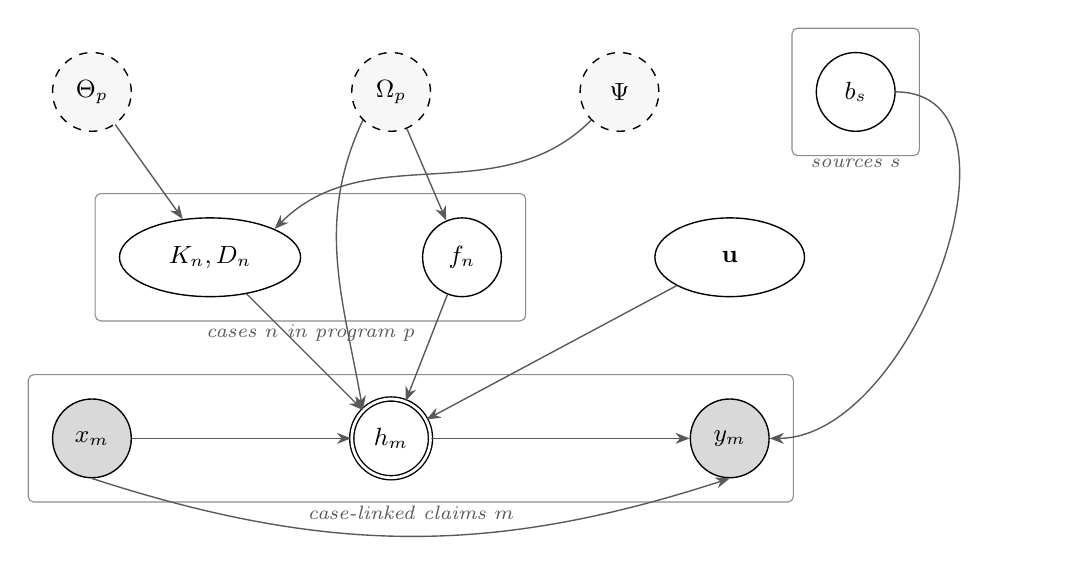
\begin{tikzpicture}[x=1cm,y=1cm]
  \node[shared] (pop) at (1.3,2.5) {$\Theta_p$};
  \node[shared] (clock) at (5.1,2.5) {$\Omega_p$};
  \node[shared] (select) at (8.0,2.5) {$\Psi$};
  \node[latent] (source) at (11.0,2.5) {$b_s$};
  \node[bundle,minimum width=23mm] (case) at (2.8,.4) {$K_n,D_n$};
  \node[latent] (fraction) at (6.0,.4) {$f_n$};
  \node[bundle] (coverage) at (9.4,.4) {$\mathbf u$};
  \node[observed] (meta) at (1.3,-1.9) {$x_m$};
  \node[derived] (operator) at (5.1,-1.9) {$h_m$};
  \node[observed] (report) at (9.4,-1.9) {$y_m$};
  \begin{scope}[on background layer]
    \node[plate,fit=(case)(fraction)] (np) {};
    \node[plate,fit=(source)] (sp) {};
    \node[plate,fit=(meta)(operator)(report)] (mp) {};
  \end{scope}
  \node[ptag,anchor=north] at (np.south) {cases $n$ in program $p$};
  \node[ptag,anchor=north] at (sp.south) {sources $s$};
  \node[ptag,anchor=north] at (mp.south) {case-linked claims $m$};
  \draw[ed] (pop) -- (case);
  \draw[ed] (clock) -- (fraction);
  \draw[ed] (select.south west) to[out=225,in=45] (case.north east);
  \draw[ed] (case) -- (operator);
  \draw[ed] (fraction) -- (operator);
  \draw[ed] (coverage) -- (operator);
  \draw[ed] (clock.south west) to[out=245,in=100] (operator.north west);
  \draw[ed] (meta) -- (operator);
  \draw[ed] (operator) -- (report);
  \draw[ed] (source.east) to[out=0,in=0] (report.east);
  \draw[ed] (meta.south) to[bend right=18] (report.south);
\end{tikzpicture}
\captionof{figure}{V5 case-report channel, conditional on source sampling context
and any known outcome. The $\Psi$ arrow denotes a normalized selected-case density,
not an agency effect. Summary and administrative-count likelihoods also use the
same population parameters, but are described below rather than drawn as cases.
Node styling follows Figure 1.}
\end{center}
\vspace{-.5em}
\begin{align*}
  \Pr(K_n=\mathrm{approval})&=\pi_p,&
  \log D_n\mid K_n=k&\sim\Normal(\mu_{pk},\sigma_p^2),\\[-2pt]
  f_n&=\logit^{-1}(\eta_p+s_f z_n),& z_n&\sim\Normal(0,1).
\end{align*}
These are \emph{population} distributions before selection; the source-conditional
density may differ. The base variant has one duration component, while the
common-preparation variant uses $s_f=0$. In sensitivity runs $s_f$ is fixed at
zero or one, not learned. Fraction and duration are conditionally independent
given program/outcome parameters in this model.

{\small
\begin{tabularx}{\linewidth}{@{}p{.22\linewidth}Y@{}}
\toprule Symbol & Definition and support \\
\midrule
$p,n,m,s,k$ & Program, case, claim, source family, and approval/denial outcome indices. \\
$\Theta_p$ & Population log-duration locations $\mu_{pk}\in\mathbb R$, spread $\sigma_p>0$, approval probability $\pi_p\in(0,1)$. \\
$K_n,D_n$ & Outcome and eventual process-start-to-initial-decision duration, in days. Known outcomes are conditioned on, not inferred again. \\
$\Omega_p$ & Preparation logit location $\eta_p$, complete-filing fraction $r_p$, closeout fraction $q_p$, and completion/progress nuisance parameters. \\
$f_n,s_f,z_n$ & Preparation fraction in $(0,1)$; fixed logit-scale heterogeneity; standard-Normal case coordinate. \\
$\Psi$ & Duration-dependent and outcome-dependent source-selection parameters, used only for applicable sampling contexts. \\
$\mathbf u,b_s$ & Partial-preparation coverage fractions; source-family log-time offsets. \\
$x_m,h_m,y_m$ & Fixed claim semantics; deterministic clock/partial-span operator; observed rounded or censored timing report. \\
\bottomrule
\end{tabularx}}

\clearpage
\section{V5 is an extension family, not several unrelated estimators}
\begin{tabularx}{\linewidth}{@{}p{.25\linewidth}YY@{}}
\toprule Class / module stem & Adds & Does not establish \\
\midrule
\code{bayes_process_}\newline\code{measurement} & Shared-case duration; clock mixtures; reporting error; optional duration selection and ambiguous completion & Agency/task timing or burden counts \\
\code{bayes_outcome_}\newline\code{measurement} & Approval/denial components; valid decided-cohort counts; outcome posting effects & Anecdotes as a population outcome survey \\
\code{bayes_preparation_}\newline\code{measurement} & Partial pre-filing spans sharing the case's total duration; disjoint-span budgets & Every span as all preparation, or overlapping spans as additive \\
\code{bayes_variable_}\newline\code{preparation} & Case-varying fractions; coherent population clock summaries; segmentation-invariant coverage option & Learned fraction heterogeneity or task-level propagation \\
\bottomrule
\end{tabularx}
The rows are successive Python subclasses, fitted through one runner. Selection,
completion and coverage settings define recorded variants, not separate posterior
ensembles. Each fit still estimates its own posterior from evidence.

\subsection*{One case, one duration, several observation operators}
For initial-decision reports, the predicted clock is $D_n$ from process start,
$(1-f_n)D_n$ from first filing, or $(1-f_n)(1-r_p)D_n$ from complete filing.
Here $r_p\in(0,1)$ removes an additional fraction of the post-first-filing clock.
Closeout adds $q_pD_n$, with $q_p>0$, to the chosen clock; it is not a new agency
service-time estimate. Unknown starts/ends use explicit prior-weighted mixtures.
First filing never means subtracting every later correction submission.

A pre-filing partial span predicts $u_m f_nD_n$. A fully anchored preparation
report has $u_m=1$. For $J$ explicitly disjoint partial spans in a group, the newer
prior is
\[
 C\sim\operatorname{Beta}(1,1),\qquad
 (v_1,\ldots,v_J)\sim\operatorname{Dirichlet}(\alpha,\ldots,\alpha),\qquad
 u_j=Cv_j.
\]
$C$ is total reported coverage, $v_j$ its allocation, $\alpha>0$ a fixed
concentration (default one), and $1-C$ unreported preparation. Total coverage no
longer increases in expectation simply because a report is split into more
pieces. Unsupported overlapping spans are not added. This use of Beta/Dirichlet
priors is for bounded nuisance fractions, not a Beta--Binomial burden model.

\subsection*{Combining reports and accounting for which cases are reported}
The contribution of one case is
\[
 L_n(\theta,f_n)=\sum_k\int_0^\infty
 p_{\mathrm{sel}}(D,k\mid\theta,x_n)
 \prod_{m\in\mathcal M_n}\ell_m(D,k,f_n;\theta)\,dD.
\]
Here $\theta$ collects model parameters, $x_n$ is known case/sampling metadata,
$\mathcal M_n$ indexes its reports, and $\ell_m$ is the appropriate clock/report
likelihood, including linked source effects. The normalized selected-case density
$p_{\mathrm{sel}}$ conditions on any known outcome (then only that $k$ contributes).
Gaussian quadrature integrates duration \emph{once per case}; its sampled
preparation fraction is shared by all reports. Selected-cohort offsets are
additional nuisance effects, suppressed in the schematic. Population summaries
instead observe functionals of the outcome/clock
mixture: the median solves its CDF equation, not an average of component medians.
Finite-sample summary error is approximated, not treated as zero.

Selected stories can favor long durations and denials. The likelihood normalizes
these selection weights within the relevant outcome/sample mixture; selection and
source bias remain weakly distinguishable in small corpora. Explicit ongoing
initial-decision cases use a survival likelihood. Unknown completion uses a
completed/partial interval-probability mixture, with uncertain progress, rather
than adding an interval probability to a survival probability. Only valid
administrative \emph{decided-case} denominators constrain population approval
prevalence. Abandonment is not a completed approval/denial.

\clearpage
\section{Computation, current goals, and integration boundary}
\subsection*{Yes: posterior learning uses Monte Carlo sampling}
Both versions use blocked \emph{elliptical slice sampling} on standard-Normal
coordinates transformed to the declared priors. V4 also uses exact categorical
updates over its finite schedule/count states and conditional/interweaving moves
to improve hierarchical mixing. V5 analytically or numerically marginalizes some
latent variables and samples the remaining parameters; its case-duration
quadrature is \emph{not} an extra collection of observed cases.

Four independent chains, rank-normalized split/folded $\widehat R$ and effective
sample sizes check Monte Carlo stability. The v5 gates require
$\widehat R\leq1.01$, bulk effective sample size at least 400 and tail effective
sample size at least 200. A separate doubled-resolution check requires maximum
tested log-likelihood change below $0.01$. Convergence, integration precision,
statistical identifiability and predictive accuracy are four different questions.

\subsection*{Measured local runtime, not an estimate of cluster speed}
The observed machine is an Apple M1 Max with 10 CPU cores and 64 GiB RAM. These
fits use CPU NumPy/SciPy plus optional native Numba kernels, not a GPU backend.
The following wall times come from saved run manifests; each fit used two chain
workers. Concurrent jobs and different likelihoods make these \emph{not} a
controlled v5-versus-v6 speed comparison.

{\small
\begin{tabularx}{\linewidth}{@{}p{.42\linewidth}Y r@{}}
\toprule Run & Work per chain & Minutes \\
\midrule
V5 preparation, common fraction & 1,500 warmup + 6,000 retained & 83.5 \\
V5 preparation, variable fraction & 1,500 warmup + 6,000 retained & 96.4 \\
V6 mixed, batched likelihood & 1,000 warmup + 2,000 retained & 8.5 \\
V6 mixed, extension & 4,000 additional retained & 17.0 \\
\bottomrule
\end{tabularx}}
Minutes measure manifest start-to-completion wall time, including setup and
reporting, not just the narrower sampler timer recorded in some manifests.
V5's two fits used 1,024 duration and 64 fraction integration nodes, with roughly
two million likelihood evaluations apiece. Extensions and prediction/diagnostic
recomputation add time. Overall development time also includes implementation,
semantic audits, benchmark-clock investigation and tests; it is not all sampling.

More available CPU cores can parallelize independent chains or replicated
datasets. Within-chain transitions remain sequential, and some reporting work is
serial. Local development is appropriate; sk3 may suit batch experiments if it
has more available CPU capacity. Its hardware/load have not been checked, so no
speedup is claimed. Compare an identical saved workload before moving runs, and
avoid multiplying many workers by many BLAS threads.

\subsection*{What these versions are for now}
V4 preserves the hierarchy/transfer experiments and their failures. V5 tests the
measurement mechanisms and preparation/selection sensitivity, not a new final
product. The integration goal is one shared visit representation with agency/task
effects and distinct elapsed, payer-work and agency-work channels. The v6 prototype
already couples counts, repeated visits, timing and labor in one posterior and
optionally separates a visit's waiting from elapsed service. It does not multiply
the v4 and v5 posteriors. These are controlled component tests, not a calibrated
full text-to-burden pipeline; source integration and broader process uncertainty
remain unfinished. Elapsed service still does not imply person-hours.

In particular, the strict v6 adapter's first pass compiled none of 146 eligible
elapsed claims without further assumptions/extensions. That is a contract/model
coverage gap, not an absence of information in the documents. A controlled mixed-
evidence test improved some counts/work estimates but worsened agency-time point
accuracy. The subsequent wait/service extension makes five of those claims
model-compatible if sampling/interpretation priors are supplied, but strict
coverage remains zero. Full-burden calibration and a clean matched-LLM comparison
remain open.

\clearpage
\section*{Source map and evaluation requirements}
This is a description of the implemented architecture, not a frozen mathematical
specification of every experiment's priors. Saved configurations and code hashes
are authoritative for individual runs. All module paths below are relative to
\code{pipeline/procbench/}; documentation paths are relative to the repository.

\begin{tabularx}{\linewidth}{@{}p{.22\linewidth}Y@{}}
\toprule Responsibility & Files to inspect \\
\midrule
Evidence / semantics & \code{evidence_contract.py}; \code{reconcile_evidence.py}; \code{audit_measurement_semantics.py}; \code{audit_case_outcomes.py}; \code{audit_preparation_clocks.py} \\
V4 elapsed / effort & \code{bayes_hierarchy.py}; \code{bayes_effort.py}; \code{run_hierarchical.py}; \code{schedule_kernel.py} \\
V5 likelihood family & \code{bayes_process_measurement.py}; \code{bayes_outcome_measurement.py}; \code{bayes_preparation_measurement.py}; \code{bayes_variable_preparation.py} \\
V5 computation & \code{run_process_measurement.py}; \code{measurement_kernel.py}; \code{phase_mixture.py}; \code{latent_gaussian.py} \\
Integration work & \code{bayes_trace_hierarchy.py}; \code{compact_visit_trace.py}; \code{compile_visit_durations.py} \\
\bottomrule
\end{tabularx}

\subsection*{Experiment records}
The architectural notes and their associated result/protocol files retain failed
diagnostics and negative comparisons:
\begin{itemize}
  \item \repo{docs/2026-09-16-bayesian-process-v4.md}{\code{docs/2026-09-16-bayesian-process-v4.md}} and
    \repo{docs/2026-09-16-bayesian-process-v4-results.md}{\code{docs/2026-09-16-bayesian-process-v4-results.md}}.
  \item \repo{docs/2026-09-16-bayesian-process-v5.md}{\code{docs/2026-09-16-bayesian-process-v5.md}} and
    \repo{docs/2026-09-16-bayesian-process-v5-results.md}{\code{docs/2026-09-16-bayesian-process-v5-results.md}}.
  \item \repo{docs/2026-09-16-bayesian-visit-clocks.md}{\code{docs/2026-09-16-bayesian-visit-clocks.md}} and
    \repo{docs/2026-09-16-bayesian-process-v6-results.md}{\code{docs/2026-09-16-bayesian-process-v6-results.md}}.
\end{itemize}
Runtime manifest directories:
\begin{itemize}
  \item Under \code{runs/bayes_v5/timing/}:\\
    \code{preparation_partition_common/} and \code{preparation_partition_variable/}.
  \item Under \code{runs/bayes_v6/integration/}:\\
    \code{mixed_joint_batched/} and \code{mixed_joint_batched_extended/}.
\end{itemize}

\subsection*{What would count as success?}
A useful extension must connect a real evidence type to a defined latent quantity
and observation operator, preserve source/case dependencies, and improve a declared
test without using hidden truth in fitting. Adding hierarchy levels merely because
they can be drawn is not sufficient. Source coverage, identifiability, prior
sensitivity, computational recovery, and held-out predictive scoring all matter.

Before claiming parity or improvement over an LLM, freeze the estimator and
estimand, use matched ledgers/sidecars and program groupings, and run fresh repeated
controls. Report per-program point errors and proper interval scores, including
failures. More independent, diverse evidence can identify parameters; more copies
or selected stories need not. Neither model can learn an unobserved decomposition
from total time alone without assumptions, regardless of the number of draws.

Legacy W1 clocks also require care: the old generated scalar uses the last
recorded decision, while some prompts/measurements refer to the first initial
decision. The documented mismatch is not permission to relabel old inputs or
replace scores after seeing them. A new benchmark must declare clocks and cohorts
before inference.

\subsection*{Computation references}
\href{https://proceedings.mlr.press/v9/murray10a.html}{Murray, Adams and MacKay
(2010), \emph{Elliptical Slice Sampling}}, describes the base sampling mechanism.
\href{https://docs.scipy.org/doc/scipy-1.16.2/tutorial/parallel_execution.html}{SciPy
1.16.2, \emph{Parallel execution support}}, describes CPU/thread behavior and
BLAS oversubscription considerations. These references do not establish calibration
of this repository's model.

\end{document}
